The given equation \eqref{eq:solutions/40/1/ques} can be expressed as 
\begin{align}
&\vec{x}^T\myvec{12 & \frac{-23}{2}\\\frac{-23}{2} & 10}\vec{x}+2\myvec{\frac{-25}{2} & 13}\vec{x}-14=0\label{eq:solutions/40/1/given}
\end{align}
where 
\begin{align}
\vec{V}&=\myvec{12 & \frac{-23}{2}\\\frac{-23}{2} & 10}\\
\vec{u}&=\myvec{\frac{-25}{2} \\ 13}\\
f&=-14
\end{align}
\begin{align}
    \det(\vec{V})&=\begin{array}{|cc|}
12 & \frac{-23}{2}\\\frac{-23}{2} & 10
\end{array}\\
\implies\det(\vec{V})&=\frac{-49}{4}\\
\implies\det(\vec{V})&<0
\end{align}
Since $\det(\vec{V})<0$ the given equation \eqref{eq:solutions/40/1/given} represents the hyperbola
The characteristic equation of $\vec{V}$ is obtained by evaluating the determinant 
\begin{align}
       \begin{array}{|c|}
V-\lambda\vec{I}
\end{array}&=0\\
   \begin{array}{|cc|}
12-\lambda & \frac{-23}{2} \\ \frac{-23}{2} & 10-\lambda
\end{array}&=0\\
\implies 4\lambda^2-88\lambda-49&=0\label{eq:solutions/40/1/eqroots}
\end{align}
The eigenvalues are the roots of equation \ref{eqroots} is given by 
\begin{align}
    \lambda_1&=\frac{22+\sqrt{533}}{2}\label{eq:solutions/40/1/eqeig1}\\
    \lambda_2&=\frac{22-\sqrt{533}}{2}\label{eq:solutions/40/1/eqeig2}
\end{align}
The eigenvector $\vec{p}$ is defined as 
\begin{align}
    \vec{V}\vec{p}&=\lambda\vec{p}\\
    \implies (\vec{V}-\lambda\vec{I})\vec{p}&=0\label{eq:solutions/40/1/eqev}
\end{align}
For $\lambda_1=\frac{22-\sqrt{533}}{2}$ ,
\begin{align}
    (\vec{V}-\lambda_1\vec{I})=\myvec{\frac{\sqrt{553}+2}{2} & \frac{-23}{2} \\\frac{-23}{2} & \frac{\sqrt{533}-2}{2}}
\end{align}
By row reduction , 
\begin{align}
    &\myvec{\frac{\sqrt{533}+2}{2} & \frac{-23}{2} \\\frac{-23}{2} & \frac{\sqrt{533}-2}{2}}\\
    &\xleftrightarrow{R_1=\frac{R_1}{\left(\frac{\sqrt{533}+2}{2}}\right)}\myvec{1 & \frac{2-\sqrt{533}}{23} \\\frac{-23}{2} & \frac{\sqrt{533}-2}{2}}\\
    &\xleftrightarrow{R_2=R_2+\frac{23}{2}R_1}\myvec{1 & \frac{2-\sqrt{533}}{23} \\0 & 0}\label{eq:solutions/40/1/eqs1}
    \intertext{Subsituting equation \ref{eqs1} in equation \ref{eqev} we get }
    &\myvec{1 & \frac{2-\sqrt{533}}{23} \\0 & 0}\myvec{v_1 \\ v_2}=\myvec{0 \\ 0}\label{eq:solutions/40/1/eqei1}
\end{align}
Where, $\vec{p}=\myvec{v_1\\v_2}$
\begin{align}
    \intertext{Let v_2=t}
    v_1&=\frac{-t(2-\sqrt{533})}{23}
    \intertext{Eigen vector $\vec{p_1}$ is given by}
    \vec{p_1}&=\myvec{\frac{-t(2-\sqrt{533})}{23} \\ t}
    \intertext{Let $t=1$, we get }
    \vec{p_1}&=\myvec{\frac{\sqrt{533}-2}{23} \\1 }\label{eq:solutions/40/1/eqp1}
\end{align}
For $\lambda_2=\frac{22+\sqrt{533}}{2}$ ,
\begin{align}
    (\vec{V}-\lambda_2\vec{I})=\myvec{\frac{2-\sqrt{553}}{2} & \frac{-23}{2} \\\frac{-23}{2} & \frac{-2-\sqrt{533}}{2}}
\end{align}
By row reduction , 
\begin{align}
    &\myvec{\frac{2-\sqrt{533}}{2} & \frac{-23}{2} \\\frac{-23}{2} & \frac{-2-\sqrt{533}}{2}}\\
    &\xleftrightarrow{R_1=\frac{R_1}{\left(\frac{2-\sqrt{533}}{2}}\right)}\myvec{1 & \frac{2+\sqrt{533}}{23} \\\frac{-23}{2} & \frac{-2-\sqrt{533}}{2}}\\
    &\xleftrightarrow{R_2=R_2+\frac{23}{2}R_1}\myvec{1 & \frac{2-\sqrt{533}}{23} \\0 & 0}\label{eq:solutions/40/1/eqs2}
    \intertext{Subsituting equation \ref{eqs2} in equation \ref{eqev} we get }
    &\myvec{1 & \frac{2+\sqrt{533}}{23} \\0 & 0}\myvec{v_1 \\ v_2}=\myvec{0 \\ 0}\label{eq:solutions/40/1/eqei1}
\end{align}
Where, $\vec{p}=\myvec{v_1\\v_2}$
\begin{align}
    \intertext{Let v_2=t}
    v_1&=\frac{-t(2+\sqrt{533})}{23}
    \intertext{Eigen vector $\vec{p_2}$ is given by}
    \vec{p_2}&=\myvec{\frac{-t(2+\sqrt{533})}{23} \\ t}
    \intertext{Let $t=1$, we get }
    \vec{p_2}&=\myvec{\frac{-\sqrt{533}-2}{23} \\1 }\label{eq:solutions/40/1/eqp2}
\end{align}
By eigen decompostion $\vec{V}$ can be represented by
\begin{align}
    \vec{V}&=\vec{P}\vec{D}\vec{P}^T\label{eq:solutions/40/1/eqsubs}
    \intertext{where }
    \vec{P}&=\myvec{\vec{p_1} & \vec{p_2}}\label{eq:solutions/40/1/eqp}\\
    \vec{D}&=\myvec{\lambda_1 & 0 \\0 & \lambda_2}\label{eq:solutions/40/1/eqD}
    \intertext{Substituting equations \ref{eqp1}, \ref{eqp2} in equation \ref{eqp} we get }
    \vec{P}&=\myvec{\frac{\sqrt{533}-2}{23} & \frac{-\sqrt{533}-2}{23} \\1 & 1}\label{eq:solutions/40/1/eqP}
    \intertext{Substituting equations \ref{eqeig1}, \ref{eqeig2} in \ref{eqD} we get}
    \vec{D}&=\myvec{\frac{22-\sqrt{533}}{2} & 0\\0 & \frac{22+\sqrt{533}}{2}}\label{eq:solutions/40/1/eqDD}
\end{align}
Centre of the hyperbola is given by 
\begin{align}
    \vec{c}&=-\vec{V}^{-1}\vec{u}\\
    \implies\vec{c}&=-\myvec{\frac{-40}{49}&\frac{-46}{49}\\\frac{-46}{49}&\frac{-48}{49}}\myvec{\frac{-25}{2} \\ 13}\\
    \implies\vec{c}&=\myvec{\frac{40}{49}&\frac{46}{49}\\\frac{46}{49}&\frac{48}{49}}\myvec{\frac{-25}{2} \\ 13}\\
    \implies\vec{c}&=\myvec{2\\1}
\end{align}
Since,
\begin{align}
    \vec{u}^T\vec{V}^{-1}\vec{u}-f = 26 > 0\label{eq:solutions/40/1/cond}
\end{align} 
there isn't a need to swap axes

In hyperbola,
\begin{align}
axes=
\begin{cases}
\sqrt{\frac{\vec{u}^T\vec{V}^{-1}\vec{u}-f}{\lambda_1}}\\ \sqrt{\frac{f-\vec{u}^T\vec{V}^{-1}\vec{u}}{\lambda_2}}
\end{cases}
\end{align}
From above equations we can say that,
\begin{align}
\sqrt{\frac{\vec{u}^T\vec{V}^{-1}\vec{u}-f}{\lambda_1}}=\frac{2\sqrt{13}}{\sqrt{22+\sqrt{533}}}\\
\sqrt{\frac{f-\vec{u}^T\vec{V}^{-1}\vec{u}}{\lambda_2}}=\frac{2\sqrt{13}}{\sqrt{\sqrt{533}-22}}
\end{align}
Now \eqref{eq:solutions/40/1/given} can be written as,
\begin{align}
    \vec{y}^T\vec{D}\vec{y}&=\vec{u}^T\vec{V}^{-1}\vec{u}-f\label{eq:solutions/40/1/fi}
    \intertext{where ,}
    \vec{y}&=\vec{P}^T(\vec{x}-\vec{c})
\end{align}
To get $\vec{y}$,
\begin{align}
\vec{y}&=\vec{P}^T\vec{x}-\vec{P}^T\vec{c}\\
    \vec{y}&=\myvec{\frac{\sqrt{533}-2}{23} & 1 \\ \frac{-\sqrt{533}-2}{23} & 1}\vec{x}-\myvec{\frac{\sqrt{533}-2}{23} & 1 \\ \frac{-\sqrt{533}-2}{23} & 1}\myvec{2\\1}\\
    \vec{y}&=\myvec{\frac{\sqrt{533}-2}{23} & 1 \\ \frac{-\sqrt{533}-2}{23} & 1}\vec{x}-\myvec{\frac{2(\sqrt{533}-2)}{23}+1  \\ \frac{2(-\sqrt{533}-2)}{23} + 1}
\end{align}
Subsituting the eqauations \eqref{eq:solutions/40/1/cond}, \eqref{eq:solutions/40/1/eqDD} in equation \eqref{eq:solutions/40/1/fi}
\begin{align}
    \vec{y}^T\myvec{\frac{22+\sqrt{533}}{2} & 0\\0 & \frac{22-\sqrt{533}}{2}}\vec{y}-26&=0
\end{align}
\begin{figure}[h]
    \centering
    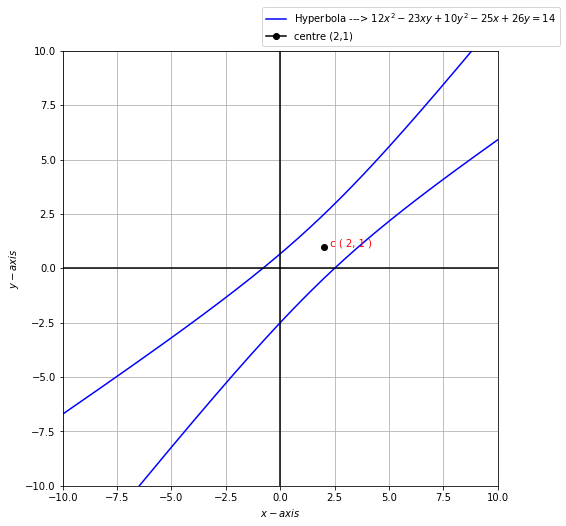
\includegraphics[width=\columnwidth]{Assignment 8.png}
    \caption{Hyperbola when origin is shifted}
    \label{eq:solutions/40/1/Fig :1}
\end{figure}

The figure \ref{eq:solutions/40/1/Fig :1} verifies the given equation \eqref{eq:solutions/40/1/given} as hyperbola with centre $\myvec{2\\1}$
